% Frame 20: SVM
\begin{frame}
    \frametitle{Support Vector Machines}
    \begin{columns}
        \begin{column}{0.5\textwidth} 
        SVMs try to solve a convex optimization problem, maximizing the distance between
        the hyperplane and the closest data points from each class. This distance is called
        "margin".
        \end{column}
        \begin{column}{0.5\textwidth} 
            \begin{figure}
                \centering
                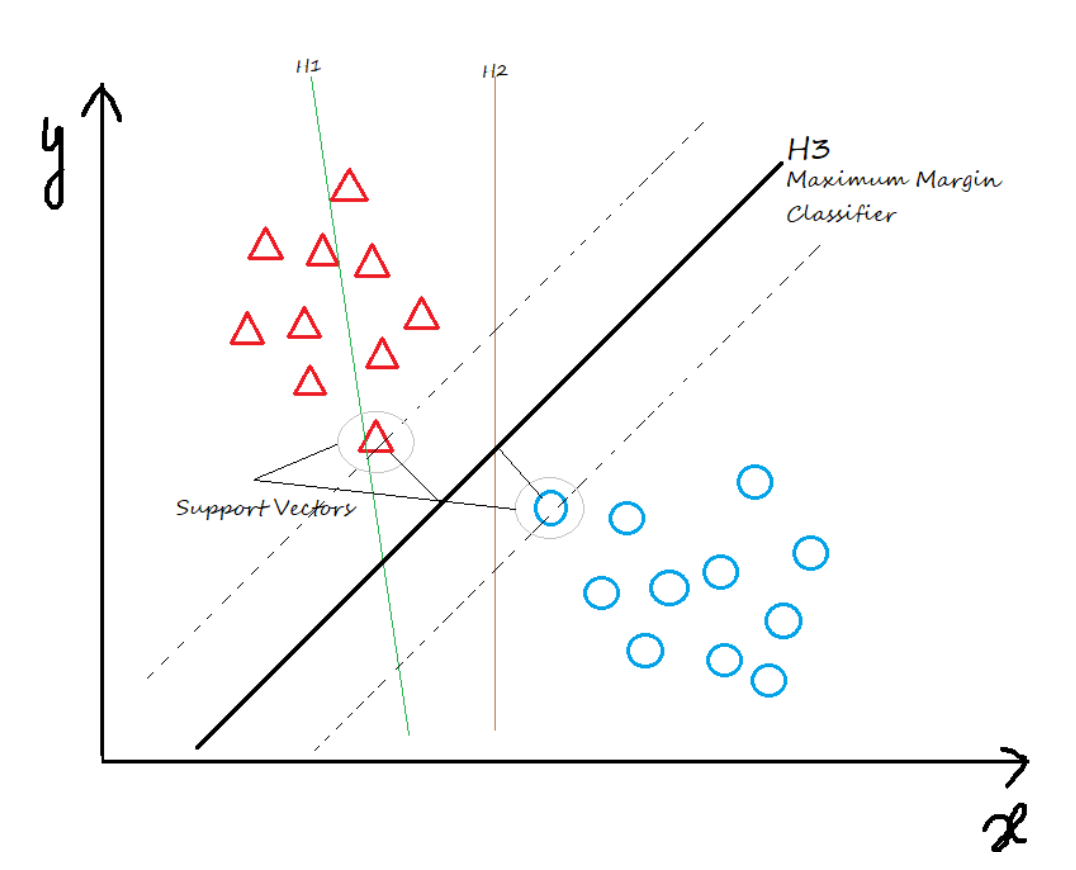
\includegraphics[width=1\textwidth]{media/2ndAssignment/svm_example.png}
                \caption{SVM}
            \end{figure}
        \end{column}
    \end{columns}
\end{frame}

% Frame 21: SVM vs MLP on hinge loss
\begin{frame}
    \frametitle{SVM vs MLP on hinge loss}
    \begin{itemize}
        \item A CPU as the training device
        \item Activation function: ReLU
        \item Loss function: Hinge loss
        \item Optimizer: Adam
        \item Learning rate: 0.001
        \item Learning rate scheduler: ReduceLROnPlateau
        \item Patience: 3 epochs
        \item Factor: 0.5
        \item Epochs: 30
        \item Training/Testing batch size: 128/256
    \end{itemize}
\end{frame}

% Frame 22: SVM vs MLP exact architectures
\begin{frame}
    \frametitle{SVM vs MLP Exact Architectures}
    \begin{columns}
        \begin{column}{0.5\textwidth} 
            The MLP model has:
            \begin{itemize}
                \item Input Flatten layer
                \item 1 hidden layer
                \item ReLU activation function
                \item 1 Dropout layer of rate of 0.3
                \item Output layer 
            \end{itemize}
        \end{column}
        \begin{column}{0.5\textwidth} 
            The SVM is just a simple one layer linear model with hinge loss. It is NOT a true SVM 
            model with margin maximization.
        \end{column}
    \end{columns}
\end{frame}

% Frame 23: SVM vs MLP graph
\begin{frame}
    \frametitle{SVM vs MLP on hinge loss}
    \begin{figure}
        \centering
        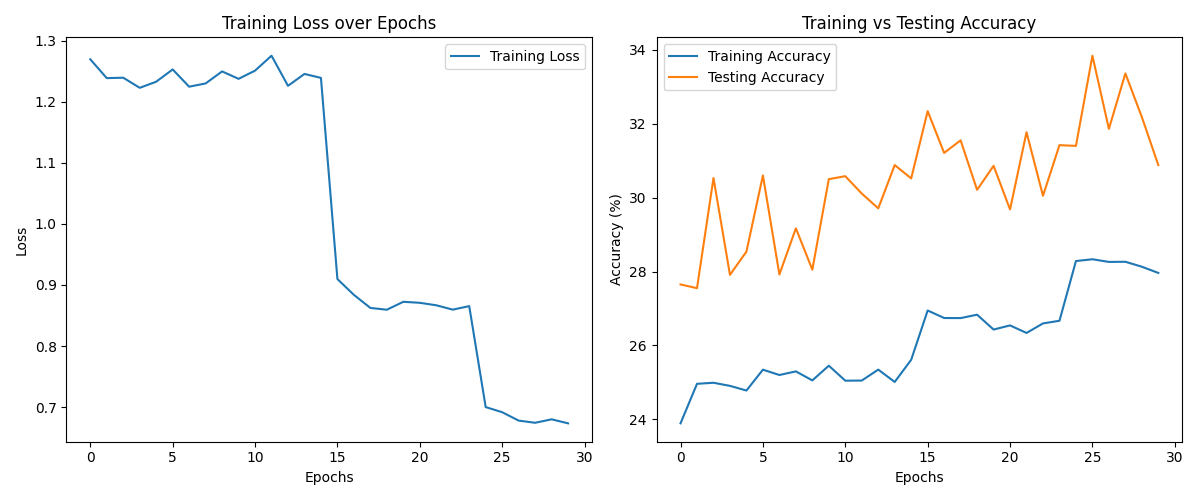
\includegraphics[height=0.4\textheight]{media/2ndAssignment/svm.png}
    \end{figure}
    \vspace{-0.5cm}
    \begin{figure}
        \centering
        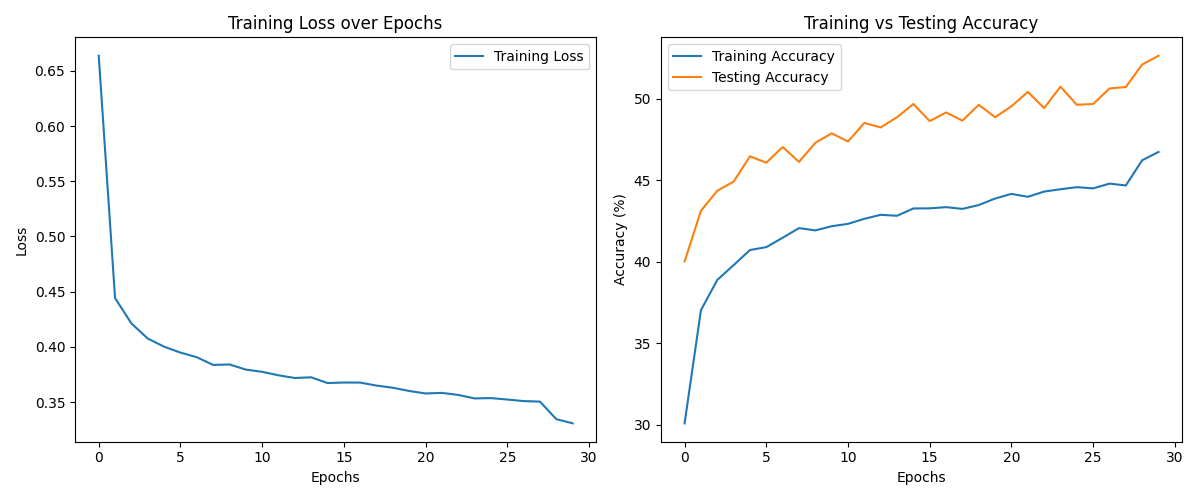
\includegraphics[height=0.4\textheight]{media/2ndAssignment/mlp.png}
        \vspace{-0.5cm}
        \caption{SVM vs MLP}
    \end{figure}
\end{frame}

% Frame 24: SVM vs MLP Results
\begin{frame}
    \frametitle{SVM vs MLP Results}
    The fake SVM model is faster but less accurate with the current configuration.
    \begin{table}[H]
        \centering
        \begin{tabular}{|c|c|c|}
            \hline
            \textbf{Model} & \textbf{Test Accuracy} & \textbf{Train Time (s)} \\ \hline % hline=horizontal line
            SVM(fake)      & 33.84                  & 321 seconds             \\ \hline
            MLP            & 52.63                  & 1184.4 seconds          \\ \hline
        \end{tabular}
        \caption{SVM vs MLP Accuracy and Training Time}
    \end{table}
\end{frame}

% Frame 25: SVM surpass KNN
\begin{frame}
    \frametitle{Attmept for the SVM to surpass the KNN}
    Transition from Adam optimizer with ReduceLROnPlateau to SGD with StepLR scheduler.\\
    Old configuration:
    \begin{itemize}
        \item Adam learning rate: 0.01
        \item ReduceLROnPlateau patience: 3
        \item ReduceLROnPlateau factor: 0.5
    \end{itemize}
    New configuration:
    \begin{itemize}
        \item SGD learning rate: 0.01 (initial)
        \item SGD weight decay: 0.0005 (penalize large weights)
        \item StepLR step size: 10 (every 10 epochs)
        \item StepLR gamma: 0.5 (reduce learning rate by half)
    \end{itemize}
\end{frame}

% Frame 26: Reality
\begin{frame}
    \frametitle{Reality}
    The fake SVM model could also have benefitted the same amount from just 
    changing the ReduceLROnPlateau factor from $factor = 0.5$ to $factor = 0.1$.
    The fixed scheduler isn't favored by the SVM as my original report suggests.\\
    \vspace{1cm}
    The tests on the second assignment were not thorough enough piling up many mistakes.
\end{frame}

% Frame 27: Real SVM
